
\chapter{语音识别中深度序列模型}
\label{chap:intro2}

最早在1990年~\cite{bourlard1989continuous,bourlard1992cdnn,bourlard2012connectionist},已经有研究者提出使用神经网络(Neural Network, NN)来对状态输出概率进行建模的方法。近几年,随着计算资源不断改善,在NN-HMM混合系统的基础上,微软研究者提出了上下文相关-深度神经网络-隐马尔可夫模型混合系统(Context-Dependent Deep-Neural-Network Hidden Markov Model, CD-DNN-HMM)~\cite{CD-DNN-HMM-dahl2012,DNN4ASR-hinton2012},即DNN-HMM混合系统,将语音识别系统性能进一步改善了相对30\%,这一系统是对传统的GMM-HMM系统的重要改进,并使得语音识别可以进行真正的商用。
另一方面,得益于分类能力有所提升,深度学习模型时序建模能力被用于搭建端到端语音识别系统。其得益于更好的序列分类能力和更简单推理框架,已经成为当前研究的热点。这类序列模型还被应用于鲁棒语音识别,通过联合优化,迁移学习,序列鉴别性训练等方式改善原来信号增强和语音识别联合训练系统。

\section{深度学习与神经网络}
\label{chap:intro2-dl}

目前语音识别领域最常使用的神经网络结构包括三种:前馈网络、卷积神经网络以及循环神经网络,本章将对这三种网络结构进行逐一介绍。在语音识别领域,深度前馈网通常简称为深度神经网络。在本文中,深度神经网络默认表示为深度前馈网络。

\subsection{深度神经网络}
神经网络~\cite{rumelhart1986learning}也被称为多层感知器,它是一种最基本神经网络结构,也是目前使用最广泛结构。深度神经网络(DNN)是一个含有很多(超过两个)隐层的多层感知器。图~\ref{fig:dnn}绘制了一个总共五层深度神经网络,包括一个输入层、三个隐层以及一个输出层。
\begin{figure}[!htp]
  \centering
    \captionstyle{\centering}
    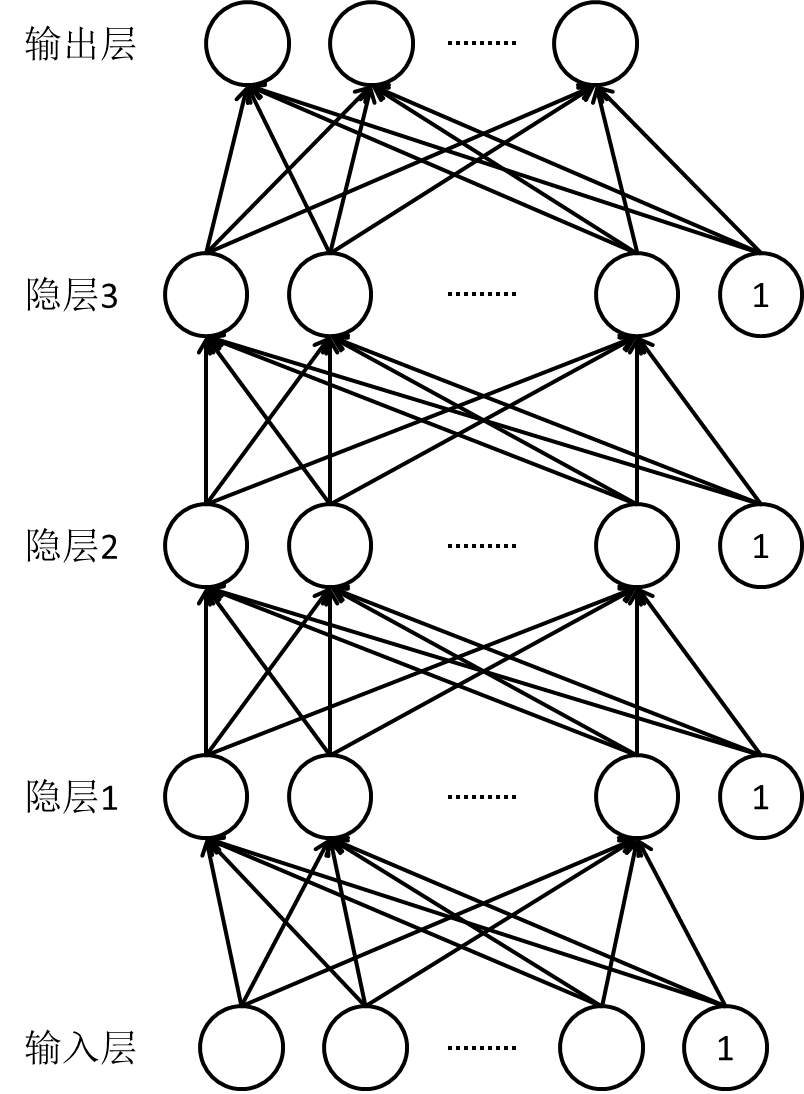
\includegraphics[height=.4\textheight]{figure/dnn.png}
    \bicaption[fig:dnn]{}{深度神经网络}{Fig}{Deep neural network}
\end{figure}
这里我们将DNN的输入层设为层0,将输出层设为层L。神经网络运算可以被定义为:
\begin{equation}
    \mathbf{y}^l=f(\mathbf{x}^l)=f(\mathbf{W}^l\mathbf{y}^{l-1}+\mathbf{b}^l), 0 < l < L
\end{equation}
这里$\mathbf{x}^l, \mathbf{y}^l, \mathbf{W}^l, \mathbf{b}^l$分别是第$l$个隐层的激励向量、激活向量、权重矩阵和偏置向量。$\mathbf{y}^0=\mathbf{o}$是网络输入特征向量。$f$是一种对激励向量进行元素级计算的激活函数。常用激活函数有:
\begin{itemize}
    \item sigmoid函数
    \begin{equation}
        \sigma(x)=\frac{1}{1+e^{-x}}
    \end{equation}
    \item 双曲正切函数
    \begin{equation}
        \text{tanh} (x)=\frac{e^x-e^{-x}}{e^{x}+e^{-x}}
    \end{equation}
    双曲正切函数是sigmoid函数的调整版本,它们具有相同建模能力。区别是sigmoid函数的值域是(0,1),这有助于得到更稀疏表示。而tanh的值域是(-1,1)是对称,更容易训练。
    \item 整流线性单元(ReLU)
    \begin{equation}
        \text{ReLU}(x)= \max (0,x)
    \end{equation}
    它的导数更加简洁且不会随着层数增多而出现梯度消失现象。
\end{itemize}
如图~\ref{fig:act}所示,其中黑色的曲线为sigmoid;红色曲线为tanh;蓝色的曲线为ReLU。因为sigmoid函数被应用得更加广泛,在本文中如果没有特别标明,默认都是使用sigmoid函数。
\begin{figure}[!htp]
  \centering
    \captionstyle{\centering}
    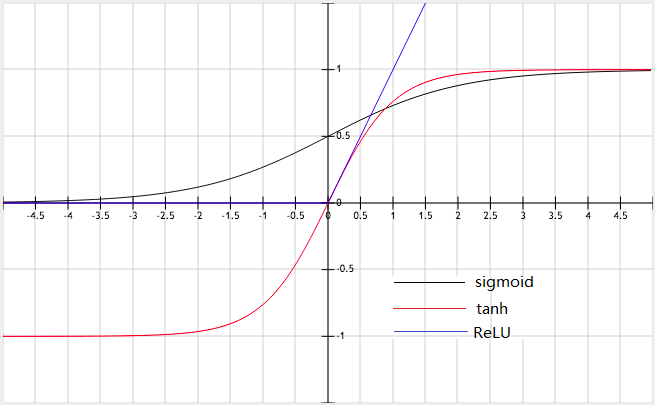
\includegraphics[height=.5\textwidth]{figure/activation.png}
    \bicaption[fig:act]{}{激活函数}{Fig}{Activation functions}
\end{figure}

深度神经网络输出层选定通常根据任务而变化,如果是回归任务,通常使用一个线性层:
\begin{equation}
    \mathbf{y}^L=\mathbf{x}^L=\mathbf{W}^L\mathbf{y}^{L-1}+\mathbf{b}^L
\end{equation}
如果是多分类的任务,通常会使用输出层每个神经元代表一类,其中第$i$个神经元的值即代表了当前特征属于类别$i$概率,因此它必须满足多项式分布,即$y^L_i \ge 0$且$\sum_{i=1}^C y_i^L=1$,这里$C$为总类别数。为了满足这一限制,我们通常会使用softmax函数进行归一化:
\begin{eqnarray}
    y_i^L&=&P_{\text{dnn}}(i|\mathbf{o})=\text{softmax}_i(\mathbf{x}^L) \\
    &=& \frac{e^{x_i^L}}{\sum_{j=1}^C e^{x_j^L}}
\end{eqnarray}
给定了特征向量的输入后,DNN输出由模型参数$\mathcal{M}=\{ \mathbf{W}^l, \mathbf{b}^l, 0 < l \le L\}$确定,通过使用前面提到的公式计算激活向量以及最后输出,这一过程也被称为前向计算。

\subsection{卷积神经网络}
传统的深度卷积神经网络(convolutional neural network, CNN)~\cite{lecun1998gradient}通常由若干卷积层和池化层组成,最后接上一些全连接层。和深度神经网络相比,它主要区别在于卷积层和池化层。本章将具体介绍卷积层和池化层。

特征图谱是卷积层和池化层中最基本的单元,每个卷积层输入和输出都是若干张特征图谱。在语音识别中,包含静态特征、一阶和二阶动态特征的经典语音信号的特征可以表示为三张特征图谱。每张特征图谱是一张大小为$N_t \times N_f$的图片,通常为$11 \times 40$。这里$N_t$是上下文窗口大小,$N_f$是提取特征的维度。相比于MFCC或者PLP特征,FBANK特征更适合CNN。首先FBANK特征中各个维度之间是相关的,这种相关性可以被卷积进行捕捉。其次,池化操作中降采样需在一个有序的频率特征图谱中进行才有意义。MFCC特征中的离散余弦变换将破坏这些性质。

\begin{figure}[!htp]
  \centering
    \captionstyle{\centering}
    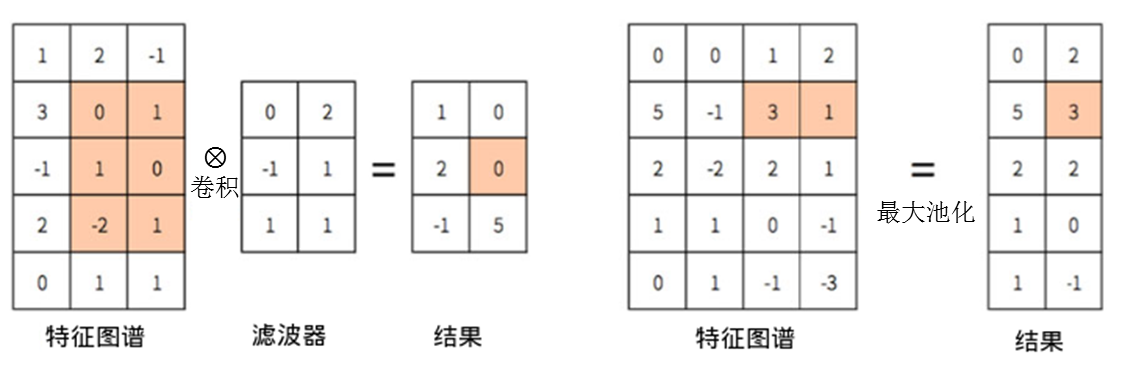
\includegraphics[width=.8\textwidth]{figure/cnn.png}
    \bicaption[fig:cnn]{卷积操作和池化操作}{卷积操作和池化操作,左边为卷积,右边为最大池化}{Fig}{Convolution and pooling, (left: convolution, right: max pooling)}
\end{figure}

卷积操作可以视为在特征图谱上使用一个滤波器。特征图谱和滤波器都可以通过矩阵表示。卷积过程就是将滤波器从特征图谱的左上角逐行扫描到右下角。在这一过程中被滤波器覆盖到的区域被称为感受野。在每一步中,感受野会将滤波器和它所覆盖到的特征图谱区域进行点乘得到一个输出值,将整张特征图谱扫描完后即可得到输出特征图谱,卷积数学定义为:
\begin{eqnarray}
    \mathbf{y} &=& \mathbf{W} \otimes \mathbf{x} \\
    y_{i,j} &=& \sum_{a=1}^A \sum_{b=1}^B W_{ab} x_{i+a-1, j+b-1} \\
    0 < &i& \le W-A+1 \\
    0 < &j& \le H-B+1 \\
\end{eqnarray}
其中$W$是大小为$A \times B$的二维滤波器,$\mathbf{x}$是大小为$W \times H$输入特征图谱,$\mathbf{y}$是大小为$W-A+1 \times H-B+1$的输出特征图谱。
如图~\ref{fig:cnn}中左边部分所示为卷积操作的图例,图中输入为一个$5 \times 3$特征图谱,滤波器大小为$3 \times 2$,最后得到一个$3 \times 2$输出特征图谱。

整个卷积层可以由如下公式表示:
\begin{equation}
    \mathbf{y}^{l}_{i} = \sigma ( \sum_{j=1}^{N} ( \mathbf{W}^{l}_{i,j} \otimes \mathbf{y}^{l-1}_{j} ) \oplus b^{l}_{i} )
\end{equation}

这里$\mathbf{y}^{l}_i, \mathbf{y}^{l-1}_j$分别是第$l$个卷积层的第$j$个输入特征图谱和第$i$个输出特征图谱。$\mathbf{W}^l_{i,j}$是这两个特征图谱间滤波器。$b^l_i$是一个应用于整张特征图谱偏置值,$\otimes$为卷积操作,$\oplus$表示特征图谱中每个元素都加上相同的值$b^l_i$。$\sigma$是激活函数,通常使用sigmoid或者ReLU。$N$是输入特征图谱个数。由于各个感受野之间的参数是共享的,因而CNN中参数个数相对DNN是很少的。

池化层通常扮演降采样功能,它输入若干特征图谱并输出降低了分辨率后特征图谱。本文使用了最大值池化方法,一个$1 \times 2$的最大值池化效果如图~\ref{fig:cnn}中的右边部分所示。

\subsection{循环神经网络}
循环神经网络(recurrent neural network, RNN)是深度神经网络一个变种,在建模时序数据中特别有效。与深度神经网络不同点在于它包含有一条回环,在循环神经网络中,隐层在时刻$t$输出不仅仅作为下一层的输入,同时也会在时刻$t+1$输回给自身。因此它相当于存在内部状态,内部状态将过去历史信息进行了编码。最简单的循环神经网络可以被描述为:
\begin{equation}
    \mathbf{y}^l_t = \sigma(\mathbf{W}^l_y \mathbf{y}^{l-1}_t + \mathbf{W}^l_h \mathbf{y}^l_{t-1} + \mathbf{b}^l)
\end{equation}
这里$\mathbf{y}^l_t$是网络第$l$层第$t$帧的隐层输出,$\mathbf{W}^l_y, \mathbf{W}^l_h$分别是用于对上层输出和对历史输出权重矩阵。

通过这一设计,神经网络可以使用所有的过去帧的信息,上下文信息在声学模型建模中扮演了很重要的作用。在~\cite{graves2013hybrid,graves2013speech,sak2014long,sak2014sequence}中,作者使用了深度循环神经网络来建模声学模型。双向循环神经网络也被用于语音识别,它不仅能捕捉过去历史信息,也能捕捉未来的整个输入序列信息。

在早期的工作中,RNN层仅仅使用了一个线性变换接上一个元素级激活函数,这种结构没法保留长时信息,因为通用的激活函数会对动态范围进行压缩,因此在$n$帧之前历史信息在到达当前帧时已经被压缩了$n$次,很难对当前决策产生影响。在使用沿时误差反向传播算法中,这一问题也被称为梯度消失问题~\cite{bengio1994learning},即误差无法沿着时间维传播太多帧。为了解决这一问题,在~\cite{hochreiter1997long}中,长短时记忆循环神经网络(long short-term memory, LSTM)被提出用来取代传统的RNN结构。它通过引入记忆单元和门操作来避免梯度消失问题,一个典型的LSTM可由如下公式描述:
\begin{eqnarray}
    \label{eq:lstm}
    \mathbf{i}^l_t &=& \sigma( \mathbf{W}^l_{yi} \mathbf{y}^{l-1}_t + \mathbf{W}^l_{hi} \mathbf{y}^l_{t-1} + \mathbf{W}_{ci} \mathbf{c}^l_{t-1} + \mathbf{b}^l_i) \\
    \mathbf{f}^l_t &=& \sigma( \mathbf{W}^l_{yf} \mathbf{y}^{l-1}_t + \mathbf{W}^l_{hf} \mathbf{y}^l_{t-1} + \mathbf{W}_{cf} \mathbf{c}^l_{t-1} + \mathbf{b}^l_f) \\
    \mathbf{c}^l_t &=& \mathbf{f}^l_t \odot \mathbf{c}^l_{t-1} + \mathbf{i}^l_t \odot \text{tanh}(\mathbf{W}_{yc} \mathbf{y}^{l-1}_t + \mathbf{W}_{hc} \mathbf{c}^l_{t-1} + \mathbf{b}^l_c) \\
    \mathbf{o}^l_t &=& \sigma( \mathbf{W}^l_{yo} \mathbf{y}^{l-1}_t + \mathbf{W}^l_{ho} \mathbf{y}^l_{t-1} + \mathbf{W}_{co} \mathbf{c}^l_{t-1} + \mathbf{b}^l_o) \\
    \mathbf{y}^l_t &=& \mathbf{o}^l_t \odot \text{tanh}(\mathbf{c}^l_t)
\end{eqnarray}
和循环神经网络一样,它需要从第一帧开始迭代进行前向传播,这里$\sigma$是非线性sigmoid函数,$\mathbf{i}^l_t, \mathbf{f}^l_t, \mathbf{o}^l_t, \mathbf{c}^l_t, \mathbf{y}^l_t$分别是第$t$帧的输入门、遗忘门、输出门、记忆单元和隐层输出。$\odot$表示元素级乘法。$\mathbf{W}_*, \mathbf{b}_*$分别是权重矩阵和偏置,其中$\mathbf{W}_{ci}, \mathbf{W}_{cf}, \mathbf{W}_{co}$是对角矩阵。与最初的LSTM结构不同之处在于,在这一结构中我们增加了窥孔连接(peephole connection)。即:将记忆单元的状态同时输入给各个门操作。

在大词汇连续语音识别任务中,按照~\cite{sak2014long}中建议,通常会使用一个投影层来降低计算量(Long Short-Term Memory with Projection, LSTMP)。它和公式~\ref{eq:lstm}的主要区别是在输出$\mathbf{y}^l_t$上增加一个线性变换来降低维度,即:
\begin{equation}
    \mathbf{y}^l_t = \mathbf{W}_{r} ( \mathbf{o}^l_t \odot \text{tanh}(\mathbf{c}_t) )
\end{equation}

\section{神经网络训练}
\subsection{训练准则}
在DNN训练中通常有两个常用的准则,对于回归任务常使用均方误差(mean square error, MSE)准则:
\begin{equation}
    \mathcal{F}_{\tt MSE}(\mathcal{M}) = \frac{1}{T}\sum_{t=1}^T \lVert \mathbf{y}_t^L - \bar{\mathbf{y}}_t \rVert^2_2
\end{equation}
这里$\mathbf{y}_t^L$是由神经网络估计出输出, $\bar{\mathbf{y}}_t$是正确标注。

对于分类任务而言,正确的标注为一个概率分布,通常使用交叉熵(cross entropy, CE)来进行优化:
\begin{equation}
    \mathcal{F}_{\tt CE}(\mathcal{M}) = - \frac{1}{T}\sum_{t=1}^T \sum_{c=1}^C \bar{y}_t(c) \log y_t^L(c)
\end{equation}
这里$\bar{y}_t(c)$是标注中类$c$概率,$y_t^L(c)$是神经网络估计出的类$c$概率。最小化交叉熵准则等价于最小化标注分布与DNN估计分布之间的KL距离(Kullback-Leibler divergence, KLD)。一般,研究者通常使用硬标注作为标注分布,即:
\begin{equation}
    \bar{y}_t(c) = 
    \begin{cases} 
        1& c=l_t \\ 
        0& c \ne l_t 
    \end{cases}
\end{equation}
这里$l_t$是第$t$帧标注。此时,CE准则退化为负对数似然准则(negative log-likelihood, NLL)
\begin{equation}
    \mathcal{F}_{\tt NLL}(\mathcal{M}) = -\log y^L_t(l_t)
\end{equation}

\subsection{反向传播算法}
给定了训练准则后,可通过著名的误差反向传播(error back-propagation, BP)~\cite{rumelhart1986learning}算法来进行参数优化。由于BP算法基于梯度下降方法来更新模型参数,因而其中的关键步骤是使用链式法则进行梯度计算。

最顶层权重矩阵的梯度取决于所使用训练准则。对于回归问题,当使用MSE的训练准则时,输出层权重矩阵的梯度是
\begin{eqnarray}
    \frac{\partial \mathcal{F}_{\tt MSE}(\mathcal{M}))}{\partial W^L_{ij}} &=& \frac{\partial \mathcal{F}_{\tt MSE}(\mathcal{M}))}{\partial x^L_j} \frac{\partial x^L_j}{\partial W^L_{ij}} \\
    &=& e^L_j \frac{\partial x^L_j}{\partial W^L_{ij}} \\
    &=& (x^L_j - \bar{y}_j) y^{L-1}_i
\end{eqnarray}
这里$e^L_j$为误差信号:
\begin{equation}
    \mathbf{e}^L \triangleq [ \frac{\partial \mathcal{F}_{\tt MSE}(\mathcal{M}))}{\partial x^L_1}, \dots, \frac{\partial \mathcal{F}_{\tt MSE}(\mathcal{M}))}{\partial x^L_N} ]^{\top}
\end{equation}
$N$是最后一层输出维度。
也可以将对$\mathbf{W}^L$梯度写为矩阵形式:
\begin{equation}
   \nabla_{\mathbf{W}^L} \mathcal{F}_{\tt MSE}(\mathcal{M})) = \mathbf{e}^L {\mathbf{y}^{L-1}}^{\top} = (\mathbf{x}^L - \bar{\mathbf{y}}) {\mathbf{y}^{L-1}}^{\top}
\end{equation}
当使用分类任务时,CE准则通常和softmax输出层一起使用,同样先计算出误差信号:
\begin{eqnarray}
    e^L_j &=& \frac{\partial \mathcal{F}_{\tt CE}(\mathcal{M}))}{\partial x^L_j} = - \frac{\partial \sum_{c=1}^C \bar{y}_c \log \text{softmax}_c(\mathbf{x}^L) }{\partial x^L_j} \\
    &=& \frac{\partial \sum_{c=1}^C \bar{y}_c \log \sum_{i=1}^C e^{x^L_i} }{\partial x^L_j} - \frac{\partial \sum_{c=1}^C \bar{y}_c \log e^{x^L_c} }{\partial x^L_j} \\
    &=& \frac{e^{x^L_j}}{\sum_{i=1}^C e^{x^L_i}} - \bar{y}_j \\
    &=& y^L_j-\bar{y}_j
\end{eqnarray}
接着可以求出对$\mathbf{W}^L$的梯度:
\begin{equation}
    \nabla_{\mathbf{W}^L} \mathcal{F}_{\tt CE}(\mathcal{M})) = (\mathbf{y}^L - \bar{\mathbf{y}}) {\mathbf{y}^{L-1}}^{\top}
\end{equation}
值得注意一点是,虽然CE准则和MSE准则梯度公式看上去有相同的形式,但实际上它们是不同的,因为在做回归时$\mathbf{y}^L=\mathbf{x}^L$,而在做分类时$\mathbf{y}^L=\text{softmax}(\mathbf{x}^L)$。

对于非顶层权重矩阵的梯度$0<l<L$,则有:
\begin{eqnarray}
    \frac{\partial \mathcal{F}(\mathcal{M}))}{\partial W^l_{ij}} &=& \frac{\partial \mathcal{F}(\mathcal{M}))}{\partial x^l_j} \frac{\partial x_j^l}{\partial W^l_{ij}} \\
    &=& e^l_j \frac{\partial x^l_jL}{\partial W^l_{ij}} \\
    &=& e^l_j y^{l-1}_i
\end{eqnarray}
这里$\mathbf{e}^l \triangleq \nabla_{\mathbf{x}^l} \mathcal{F}(\mathcal{M})$是对第$l$层的激励误差信号:
\begin{eqnarray}
    e^l_i &=& \frac{\partial \mathcal{F}(\mathcal{M})}{\partial x^l_i} \\
    &=& \sum_{j=1}^{N^{l+1}} \frac{\partial \mathcal{F}(\mathcal{M})}{\partial x^{l+1}_j} \frac{\partial x^{l+1}_j}{\partial y^l_i} \frac{\partial y^{l}_i}{\partial x^l_i} \\
    &=& \sigma'(x^{l}_i)  \sum_{j=1}^{N^{l+1}} e^{l+1}_j W^{l+1}_{ji}
\end{eqnarray}
这里$N^{l+1}$是第$l+1$层隐层节点数,写出矩阵形式即:
\begin{equation}
    \label{eq:error_prop}
    \mathbf{e}^l = ( {\mathbf{W}^{l+1}}^{\top} \mathbf{e}^{l+1} ) \odot \sigma'(\mathbf{x}^l)
\end{equation}
这里$\odot$为元素级相乘,$\sigma'(x^l_j)$为激活函数的元素级导数,对于sigmoid函数,它等于:
\begin{equation}
    \sigma'(x^l_j)=(1-y^l_j)y^l_j
\end{equation}
对于ReLU,它等于
\begin{equation}
    \sigma'(x^l_j)=
    \begin{cases}
        1& x^l_j > 0 \\
        0& x^l_j \le 0
    \end{cases}
\end{equation}
令$\sigma'(\mathbf{x}^l) = [\sigma'(x^l_1), \dots, \sigma'(x^l_{N^l})]^{\top}$。

因此对权重矩阵梯度矩阵形式为:
\begin{equation}
    \nabla_{\mathbf{W}^l} \mathcal{F}(\mathcal{M}) = \mathbf{e}^l {\mathbf{y}^{l-1}}^{\top}
\end{equation}
从公式\ref{eq:error_prop}中可以观察到,误差信号需要自顶层向下进行反向传播,因此该方法被称为误差反向传播算法。

\subsection{小批量随机梯度下降}
深度神经网络采用梯度下降的方法进行优化,因此每一轮迭代都需要对一个批量(batch)训练样本计算梯度。批量大小的选择上通常海会同时影响收敛速度与模型的性能。

最简单批量选择方法是去使用整个训练集,这种方法被称为批量训练(batch training)。它有如下优势:首先,批量训练的收敛性是众所周知的,其次,批量训练可以在多计算机之间并行。但由于每次参数更新都要遍历全部数据集~\cite{yu2010roles},所以对大词汇语音识别任务而言,这是十分低效的。

另外一种选择是随机梯度下降法(Stochastic gradient decent, SGD)~\cite{bottou1998online},在机器学习领域也被称作在线学习。SGD根据从单个训练样本估计出的梯度来更新模型参数~\cite{yu2010roles}。如果样本点是独立同分布的(在训练数据中随机采样很容易达成),可以证明这种方法是对梯度的无偏估计,只不过存在噪声。这点虽然看似不利,实则是SGD相比批量算法优势所在:由于DNN是高度非线性的且优化准则也是非凸的,因而目标函数包含很多局部最优,而SGD估计中存在噪声,从而使得其能从局部最优中跳出来进入一个更好全局最优。

SGD通常比批量训练快很多,特别是在大词汇连续语音识别中。这是因为在大数据集中,通常有很多样本是相似甚至重复的,所以用全部数据集来计算梯度是浪费的。然而,由于SGD只计算一个样本梯度,无法高效的利用GPU的并行能力,且因为噪声的存在无法完全收敛至局部最优点,所以通常会使用SGD和批量训练折中方案,小批量(mini-batch)训练~\cite{yu2010roles}。小批量数据通过从训练样本中抽取一小组数据来计算梯度使得其可以高效的使用GPU的并行能力,并且也拥有SGD跳出局部最优的性质。

\subsection{惯性系数}
惯性系数~\cite{polyak1964some}是优化中一种加速收敛的方法,它主要思想是使用过往梯度的一个累积量和当前梯度的插值作为最终更新使用的梯度,即:
\begin{eqnarray}
    \Delta\mathbf{W}^l_p = \rho \Delta \mathbf{W}^l_{p-1} + (1-\rho) \frac{1}{M} \sum_{m=1}^M \nabla_{\mathbf{W}^l_p} \mathcal{F}(\mathcal{M}, \mathbf{o}_m, \bar{\mathbf{y}}_m)
\end{eqnarray}
这里,$\nabla_{\mathbf{W}^l_p} \mathcal{F}(\mathcal{M}, \mathbf{o}_m, \bar{\mathbf{y}}_m)$是使用样本$\mathbf{o}_m, \bar{\mathbf{y}}_m$计算出的梯度。$\Delta\mathbf{W}^l_p$是第$p$轮迭代累积的梯度。$\rho$即为惯性系数。使用惯性系数会令参数更新变得更加平滑,同时减少梯度估计时方差,因此可以加速训练。

\subsection{参数初始化与预训练}
通常有很多启发式的方法来初始化DNN模型,它们的主要思想都是希望初始化后的激活范围处于sigmoid函数的线性段。即激活值为0.5左右。如果权重过大将导致激活值趋近于0或者1,这样计算出梯度就会非常小。随机初始化的另外一个作用是打破深度神经网络的对称性。在~\cite{lecun1998efficient}中,Lecun建议从一个均值为0,方差为$\frac{1}{\sqrt{N^l}}$的高斯分布中采样。由于在语音识别中隐层节点的个数通常从1000至2000不等,所以一般选取[-0.05, 0.05]的均匀分布作为权重矩阵的初始化,而偏置初始化为0。

由于DNN模型高度非线性和非凸性,研究者通常会使用一些预训练的方法使其能从一个更优的初始值开始优化。最著名的两个预训练方法是深度置信网络和鉴别性预训练。

\subsubsection{深度置信网络}
深度置信网络(Deep belief network, DBN)是由多层受限玻尔兹曼机(restricted Boltzmann machine, RBM)组成生成性模型。

\begin{figure}[!htp]
  \centering
    \captionstyle{\centering}
    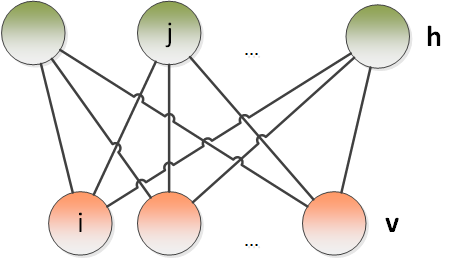
\includegraphics[width=.5\textwidth]{figure/RBM.png}
    \bicaption[fig:rbm]{}{受限玻尔兹曼机}{Fig}{Restricted Boltzmann machine}
\end{figure}

受限玻尔兹曼机是一种生成性模型,它是玻尔兹曼机的一个变种。它结构如~\ref{fig:rbm}所示~\footnote{图片引用自~\cite{ASRBook-Yu2014}},它取消了玻尔兹曼机中可见层神经之间和隐藏层神经之间的连接。因此,它形成了一张二分图。

RBM对于每一对给定隐藏层向量$\mathbf{h}$和可见层向量$\mathbf{v}$定义了一个能量函数:
\begin{equation}
    E(\mathbf{v}, \mathbf{h}) = -\mathbf{a}^{\top} \mathbf{v} - \mathbf{b}^{\top} \mathbf{h} - \mathbf{h}^{\top} \mathbf{W} \mathbf{v}
\end{equation}
这里$\mathbf{W}$是连接可见层和隐藏层之间的权重矩阵,$\mathbf{a}$和$\mathbf{b}$分别是可见层和隐藏层的偏置向量。如果可见层值域是实数域,那么能量函数定义为:
\begin{equation}
    E(\mathbf{v}, \mathbf{h}) = \frac{1}{2}(\mathbf{v}-\mathbf{a})^{\top} (\mathbf{v} - \mathbf{a}) - \mathbf{b}^{\top} \mathbf{h} - \mathbf{h}^{\top} \mathbf{W} \mathbf{v}
\end{equation}
定义完能量函数后可以定义可见向量和隐藏向量的联合概率分布:
\begin{equation}
    P(\mathbf{v}, \mathbf{h}) = \frac{e^{-E(\mathbf{v}, \mathbf{h})}}{Z}
\end{equation}
这里$Z=\sum_{\mathbf{v},\mathbf{h}} e^{-E(\mathbf{v}, \mathbf{h})}$被称为配分函数(partition function)。

在RBM中,由于隐层神经元之间没有连接,因而可见层神经元之间也没有连接~\cite{yu2010roles}。所以,可以很方便计算后验概率$P(\mathbf{v}|\mathbf{h})$和$P(\mathbf{h}|\mathbf{v})$:
\begin{eqnarray}
    P(\mathbf{h}|\mathbf{v}) &=& \frac{e^{-E(\mathbf{v}, \mathbf{h})}}{\sum_{\bar{\mathbf{h}}}e^{-E(\mathbf{v}, \bar{\mathbf{h}})}} \\
    &=& \frac{\prod_i e^{b_ih_i+h_i\mathbf{w}^{\top}_i \mathbf{v}}}{\prod_i \sum_{\bar{h}_i} e^{b_i\bar{h}_i+\bar{h}_i\mathbf{w}^{\top}_i \mathbf{v}}} \\
    &=& \prod_i P(h_i|\mathbf{v})
\end{eqnarray}
这里$\mathbf{w}^{\top}_i$是矩阵$\mathbf{W}$的第$i$行,该公式表明在给定可见层向量后,隐藏层神经元之间是条件独立的,且:
\begin{equation}
    P(h_i=1 | \mathbf{v}) = \frac{e^{b_i+\mathbf{w}^{\top}_i \mathbf{v}}}{e^{b_i+\mathbf{w}^{\top}_i \mathbf{v}} + 1} = \sigma(b_i + \mathbf{w}^{\top}_i \mathbf{v})
\end{equation}
这里$\sigma$是sigmoid函数。同样,我们可以推导出二进制可见层神经元后验概率:
\begin{equation}
    P(\mathbf{v}|\mathbf{h})=\sigma(\mathbf{W}^{\top}\mathbf{h}+\mathbf{a})
\end{equation}
对于实数可见层神经元,有:
\begin{equation}
    P(\mathbf{v}|\mathbf{h}) = \mathcal{N}(\mathbf{v}; \mathbf{W}^{\top}\mathbf{h}+\mathbf{a}, I)
\end{equation}
将多个RBM网络自底向上逐层堆叠就得到了深度信念网络,在深度信念网络中每一层的输出都作为后一层的输入,然后用新特征继续训一个RBM。最终DBN训练完成后将DBN中的权重直接作为DNN网络初始化。

使用DBN进行预训练有如下潜在优势:
\begin{itemize}
    \item DNN是高度非线性且非凸的,初始化点会很大程度影响最终模型。
    \item 预训练阶段使用的是生成性准则与反向传播算法中使用的鉴别性准则不同~\cite{yu2010roles},因此潜在对模型进行了正则化。
    \item 在预训练时可以利用大量的无标注数据。
\end{itemize}

\subsubsection{鉴别性预训练}
DNN的参数也可以使用鉴别性预训练(discriminative pretrain, DPT)来鉴别性地初始化,即逐层进行BP。鉴别性预训练流程如下: 首先使用标注鉴别性训练一个单隐藏层的DNN若干轮(并不需要训练到收敛),接着在最后一个隐层和输出层之间插入一个新的随机初始化的隐藏层,并且鉴别性训练整个网络若干轮,直至达到期望的层数。预训练目标是希望网络能从一个更优秀的初试点开始进行训练以潜在地改善神经网络鲁棒性。然而,当训练数据足够大(大于15小时)或者使用ReLU作为激活函数之后,预训练带来性能提升就不那么明显了。

\section{深度神经网络-隐马尔可夫模型混合系统}

\label{sec:dnn_hmm}

\begin{figure}[!htp]
  \centering
    \captionstyle{\centering}
    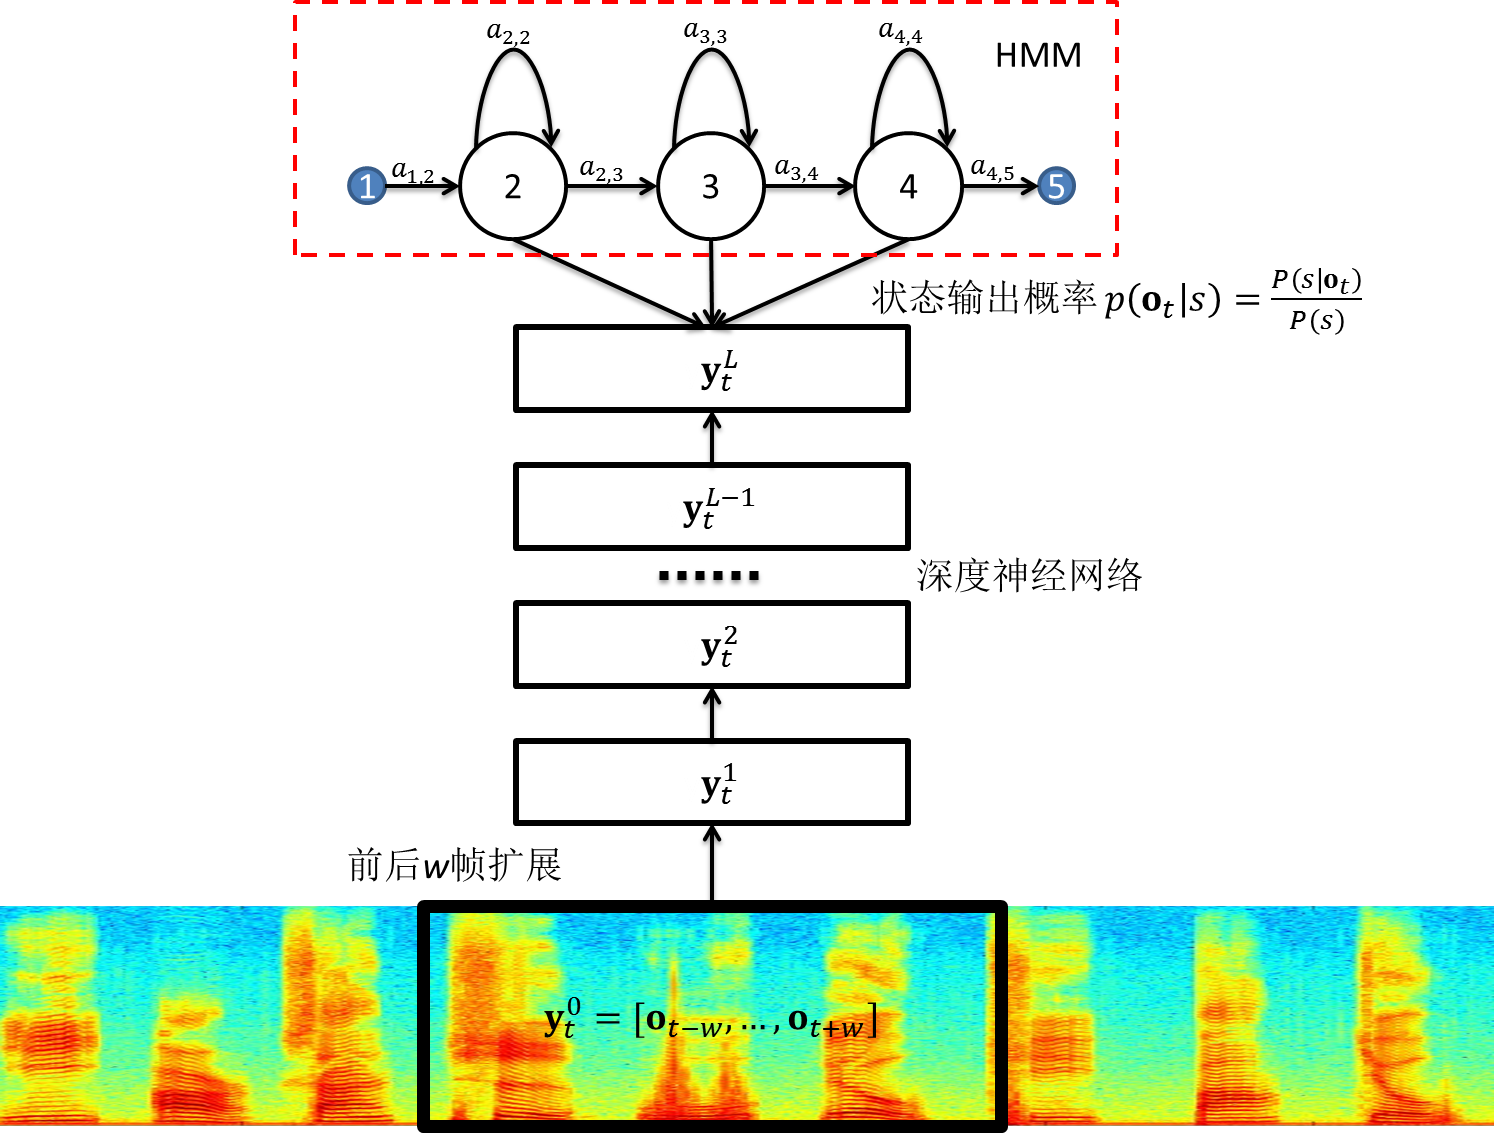
\includegraphics[width=.618\textwidth]{figure/dnn_hmm.png}
    \bicaption[fig:dnn-hmm]{}{DNN-HMM混合系统}{Fig}{Structure of DNN-HMM hybrid system}
\end{figure}

在前文介绍的深度神经网络并不能直接为语音信号的信号建模,这是由于语音信号处理的信号是一种时序连续信号,而深度神经网络的输入是固定大小的向量。早在20世纪80年代末就已经有研究提出了结合人工神经网络(ANN)和HMM方法用于语音识别~\cite{trentin2001survey}。目前有效的方法是如图\ref{fig:dnn-hmm}中所描绘的DNN-HMM混合系统。在这一框架中,HMM被用于描述语音信号的信号动态变化,而DNN则用于估计语音信号的特征向量的输出概率,通常是用来估计给定观测语音信号的特征后,该特征由HMM中某个状态释放后验概率。DNN-HMM的优点在于它能方便的利用DNN内在的鉴别性能力,另外训练过程可以直接使用维特比算法,解码过程不需要有特别改变。

在~\cite{bourlard1989continuous,bourlard1989links,morgan1990continuous}中,该方法被称为ANN-HMM混合模型,它只使用了上下文无关音素状态之间且仅用于小词汇语音识别。随后在~\cite{bourlard1992cdnn}中被扩展为上下文相关的音素建模,以及被用于LVCSR任务~\cite{robinson2002connectionist}。但是,因为过去计算能力有限,通常只使用了两层隐层的神经网络,所在并没有比GMM-HMM框架取得更好性能。

最近的技术发展~\cite{CD-DNN-HMM-dahl2012,DNN4ASR-hinton2012,seide2011conversational,yu2010roles}则说明,如下几个改变可以使其获得更重大识别性能提升。
\begin{itemize}
    \item 首先,使用更深的深度神经网络,比如拥有6个隐层DNN。
    \item 其次,使用语素(即状态聚类后的三音素状态)来代替单音素状态作为深度神经网络的输出单元。这一模型被称为上下文相关的深度神经网络隐马尔可夫模型(Context-dependent pre-trained deep-neural-network hidden markov model, CD-DNN-HMM)。直接使用语素还有一个额外好处,即它对CD-GMM-HMM系统修改最小。
\end{itemize}
在CD-DNN-HMM中。对于所有的状态$s \in [1,S]$中只有一个完整的DNN来估计状态后验概率$P(s_t=s|\mathbf{o}_t)$。这和传统的GMM是不同的,在GMM中,我们使用不同GMM来对不同的状态建模。除此之外,典型的DNN输入不是单独一帧,而是一个$2w+1$帧大小窗口特征$\mathbf{y}^0_t= [ \mathbf{o}_{t-w}^{\top}, \dots, \mathbf{o}^{\top}_t, \dots, \mathbf{o}^{\top}_{t+w} ]^{\top}$

在解码过程中,因为HMM需要使用似然度$p(\mathbf{o}_t|s_t)$而非后验概率,所以我们需要将后验概率转为似然度:
\begin{equation}
    \label{eq:dnn}
    p(\mathbf{o}_t|s_t=s) = \frac{P(s_t=s|\mathbf{o}_t)p(\mathbf{o}_t)}{P(s)}
\end{equation}
其中,$p(s)=\frac{T_s}{T}$是从训练集中统计出的每个状态先验概率。$T_s$是状态$s$的帧数,$T$是总帧数。因为$p(\mathbf{o}_t)$是与词序列无关的,计算时可忽略。所以最终似然可以通过$p(\mathbf{o}_t|s_t=s)=\frac{P(s_t=s|\mathbf{o}_t)}{P(s)}$计算。

CD-DNN-HMM训练可以使用维特比算法来进行,CD-DNN-HMM包含了三个组成部分,深度神经网络DNN,隐马尔可夫模型HMM和GMM-HMM系统中的状态绑定结构的状态。所以CD-DNN-HMM第一步是去使用训练数据训练一个GMM-HMM,然后在该系统上使用维特比算法获得状态级的强制对齐,同时保留该系统中的状态转移概率和状态映射关系,接着使用由GMM-HMM系统计算得到状态对齐(state alignment)作为标注使用CE准则训练一个DNN。最后,解码时使用公式~\ref{eq:dnn}来得到似然进行解码。


\section{端到端语音识别中的深度序列模型}
\label{chap:intro2-e2e}

得益于标注数据的增多和算力改善,深度学习模型取得了更强的分类能力。由此人们开始考虑直接使用深度序列模型对序列进行直接建模,以取得更好序列建模能力。如图~\ref{fig:e2e-idea}所示,原来传统系统中的tri-phone HMM状态建模可以直接被深度模型所取代,由此直接对音素序列进行建模。

\begin{figure}[!htp]
  \centering
    \captionstyle{\centering}
    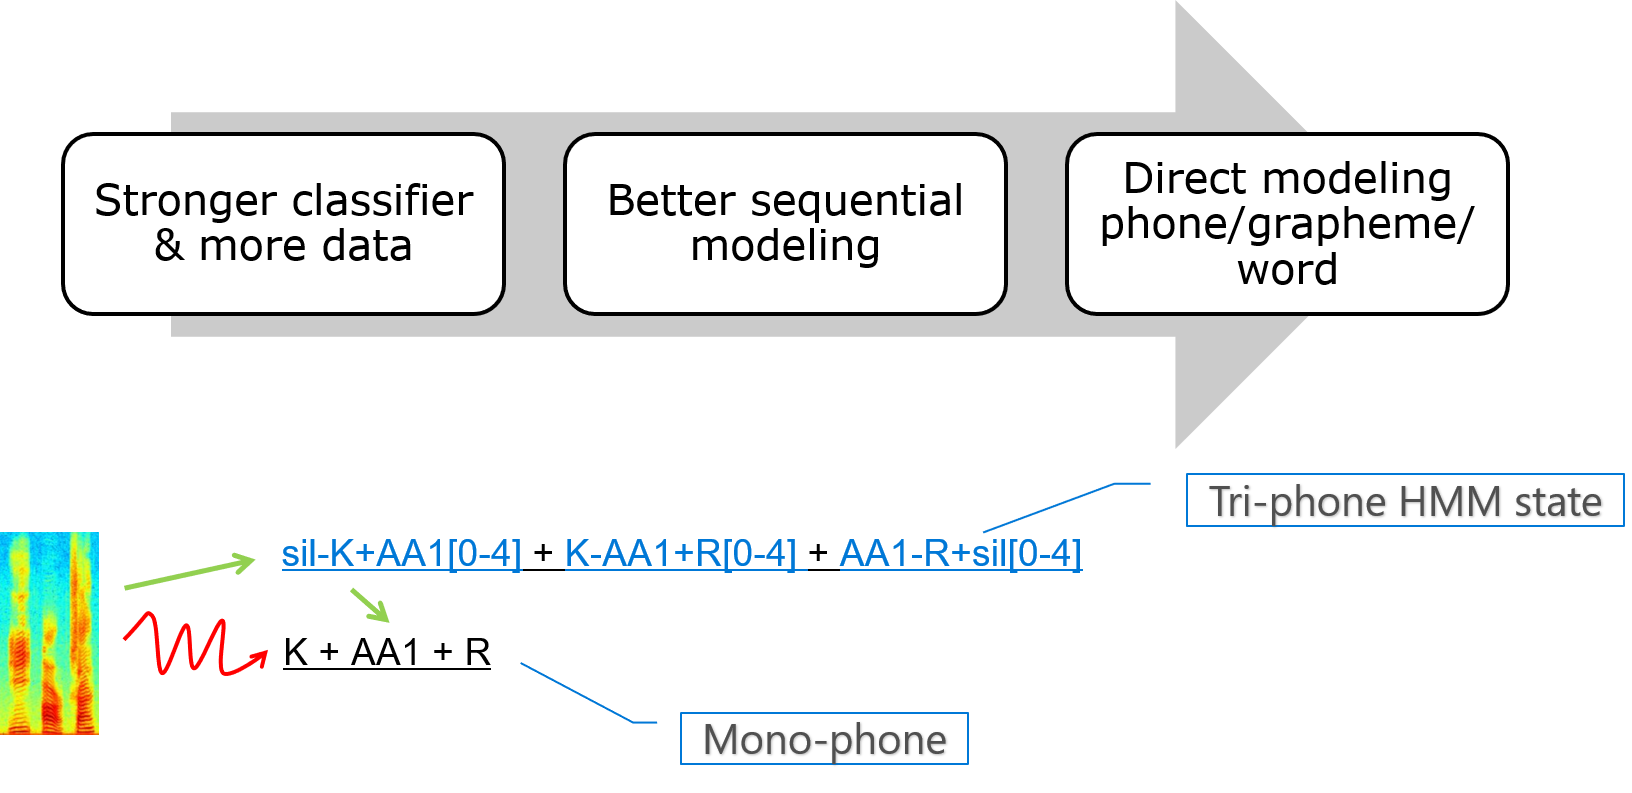
\includegraphics[clip=true, width=0.8\textwidth]{figure/e2e-idea.png}
    \bicaption[fig:e2e-idea]{}{端到端系统举例}{Fig}{Motivation and Example of End-to-end Modeling}
\end{figure}

图~\ref{fig:e2e}给出了一系列端到端序列建模模型,下文中将逐一进行讨论。

\subsection{无词图鉴别性训练模型}
\label{chap:intro2-e2e-lfmmi}

无词图鉴别性训练({\em lattice-free maximum mutual information}, LF-MMI~\cite{povey2016purely,chen2006advances})是指使用一个预先剪枝过的音素语言模型来代替传统鉴别性训练中词图。
该语言模型用于建模鉴别性训练中的搜索空间。

训练阶段依据公式\ref{equ:kws-mmi}计算声学模型序列后验概率,表示为 $\tt{LF\text{-}MMI}$。
\begin{equation}
\label{equ:kws-mmi}
\begin{split}
\mathcal{F}_{\tt{LF\text{-}MMI}}
%=- \sum_{u} \log \frac {p(\mathbf{O}_u|\mathbf{S}_u)^{\kappa}P(\mathbf{W}_u)}{\sum_{\mathbf{W}} p(\mathbf{O}_u|\mathbf{S})^{\kappa}P(\mathbf{W})}  
=\sum_{u} \log \frac {\sum_{\mathbf{L}_u} p(\mathbf{O}_u|\mathbf{L}_u)^{\kappa}P(\mathbf{L}_u)}{\sum_{\mathbf{L}} p(\mathbf{O}_u|\mathbf{L})^{\kappa}P(\mathbf{L})}  
\end{split}
\end{equation}
在公式中, $\mathbf{L}$ 是由音素组成的发音序列, $\mathbf{L}_u$ 是标注序列,也由音素组成。
$p(\mathbf{O}_u|\mathbf{L})$ 和 $p(\mathbf{O}_u|\mathbf{L}_u)$由HMM模型公式定义得到。 


该方法与传统鉴别性训练不同之处在于: 
\begin{itemize}
\item 在分母式子中所使用的标注序列 $\mathbf{L}_u$ 存在多种候选路径,这些候选路径来自于标注软对齐中对标签在一定窗宽内左右帧移。这里将所有可能的对齐路径都存储在分子词图中。
\item 模拟搜索空间分母语言模型 $P(\mathbf{L})$, $P(\mathbf{L}_u)$是使用一个在训练标注文本中训练得到的音素语言模型。
\item 一个专用HMM拓扑结构被专门提出,它包含有两个HMM状态。其中状态${\bf q}_2$ 用于模拟CTC中的$\tt blank$ 建模单元,同时其他状态来模拟输出标签单元。这里不同之处在于每个 tri-phone都维护一个它专有的$\tt blank$建模。
\item 输出帧率被降低了3倍。
\end{itemize}


\begin{figure}[!htp]
  \centering
    \captionstyle{\centering}
    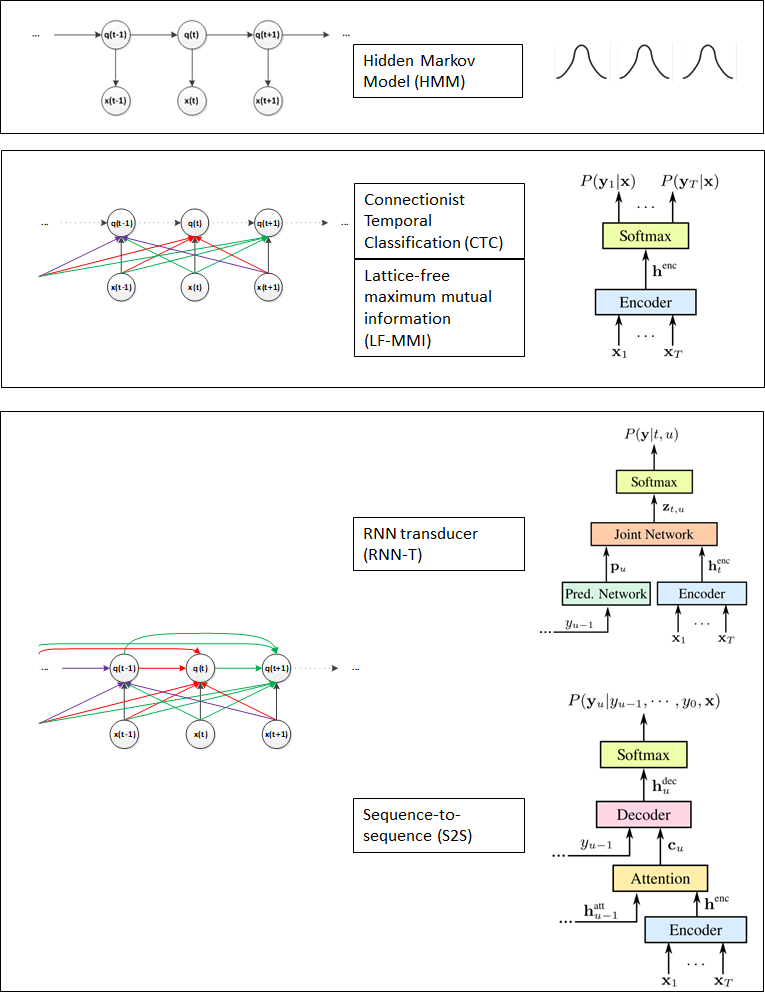
\includegraphics[clip=true, width=0.9\textwidth]{figure/e2e.png}
    \bicaption[fig:e2e]{}{传统系统与端到端系统比较}{Fig}{Comparison of Various End-to-end Models}
\end{figure}


\subsection{连接时序模型}
\label{chap:intro2-e2e-ctc}

对于DNN-HMM混合模型而言,我们通常选取帧层面的交叉熵函数作为代价函数对DNN模型进行更新,这个过程中预先需要由GMM模型提供训练语料的帧层面的对齐。连接时序模型(Connectionist Temporal Classification, CTC)提出自动学习输入帧特征序列与其对应标签序列之间的对齐关系。

我们可以预先定义训练集的标签序列包含K个不同标签,这其中还包含意味着无发射标签的空符号标签$\tt blank$建模单元。我们定义输入帧特征序列以及相对应的标签序列。这样我们就可以通过在给定输入序列的条件下最大化标签序列的对数似然比对前端预测模型进行更新。

然而由于标签并不是对齐到帧层面的,因此我们无法直接计算该似然比。为了建立前端预测模型输出与标签序列之间联系,
CTC模型被定义为标注序列在给定特征序列后的后验概率 $P(\mathbf{L}|\mathbf{O})$。
CTC引入上述 $\tt blank$ 状态来对标签之间的混淆区段进行建模。具体来说,模型在标注$l_{i-1}$ 和 $l_{i}$之间,通常预测出 $ \tt blank$ 标注。

\begin{equation}
\label{equ:ctc-model}
\begin{split}
P(\mathbf{L}|\mathbf{O})=\sum_{\mathbf{q}\in\mathcal{B}(\mathbf{L})}P(\mathbf{q}|\mathbf{O}) =\sum_{\mathbf{q}}\prod_{t=1}^{T} p(q_t|\mathbf{O})
\end{split}
\end{equation}
公式中 $\mathcal{B}$ 是一个一对多的映射函数~\footnote{在最早文献~\cite{graves2006connectionist}中使用的公式定义为一个多对一映射函数,同时使用它的反函数来定义 $\mathcal{B}^{-1}(\cdot)$ CTC模型中的映射。这里我们修改为一个一对多映射函数,使公式与HMM中的定义更加一致。}:
\begin{equation}
\label{equ:ctc-b}
\begin{split}
\mathcal{B}:\mathbb{L}   \mapsto  \mathbb{L} \cup \{\tt blank\}
\end{split}
\end{equation}
$\mathcal{B}$ 决定了标签序列 $\mathbf{L}$ 和它相应由建模单元所组成的模型状态序列$\mathbf{q}$。 这一映射做法是在每个组成 $\mathbf{L}$ 的$l$的标签中,插入一个可选并且可重复的 $ \tt blank$ 标签。 $P(q_t|\mathbf{O})$是由深度学习模型直接根据给定的特征序列$\mathbf{O}$来估计得出的, 比如使用LSTM~\cite{hochreiter1997long}。 

\subsection{基于注意力机制序列到序列模型}
\label{chap:intro2-e2e-s2s}

另一类端到端模型称为序列到序列模型。下文讨论将以基于注意力机制的序列到序列模型~\cite{chan2016end}为主进行介绍,该类模型也是当前主要研究热点。
该模型预测了在直接给定特征序列$\mathbf{x}$下的标签序列和之前已经预测出的标签历史序列$\mathbf{l}_{1:i-1}$后验概率。
\begin{equation}
\vspace{-0.6em}  
\label{equ:enc-dec}
\begin{split}
P(\mathbf{l}|\mathbf{x})=\prod_i P(l_{i}|\mathbf{x},\mathbf{l}_{1:i-1})
\end{split}
\end{equation}
%An attention mechanism weights  hidden vectors of the audio feature sequence to pick the most related hidden vectors for prediction at every step of the output sequence.
\begin{equation}
%\vspace{-0.6em}
\label{equ:enc-dec-hid}
\begin{split}
\mathbf{h}&=\text{Encoder}(\mathbf{x})\\
\end{split}
\vspace{-0.3em}  
\end{equation}
\begin{equation}
\label{equ:enc-dec-dec}
P(l_{i}|\mathbf{x},\mathbf{l}_{1:i-1})=\text{AttentionDecoder}(\mathbf{h}, s_{i-1})
\end{equation}
在公式中, $\mathbf{h}$表示编码器(encoder)网络的隐层状态。$\mathbf{s_{i-1}}$表示解码器(decoder)的上一输出相应隐层状态。$\text{Encoder}(\cdot)$ 通常是一个单向或者多向的LSTM网络,同时 $\text{AttentionDecoder}(\cdot)$ 通常是一个单向LSTM网络。 %\addcomment{this notation is not clear, does $\mathbf{x}$ mean all features in th sequence? why subscript for time in $\mathbf{l}$ but superscript for $\mathbf{s}$ }

与传统混合系统~\cite{hinton2012deep}相比,该模型所使用的$\text{AttentionDecoder}(\cdot)$隐含地建模了语言模型信息,并将其与 $\text{Encoder}$所组成声学模型进行联合训练。
%
%In the inference stage, AttentionDecoder uses hypotheses from previous steps and weighted average of encoder outputs to predict the next label. 
%
%Beam search is always applied to constrain the search space.
%
由于该模型中的声学模型和语言模型进行了紧密的联合训练,这种端到端系统并不容易被自适应到新的领域或者上下文环境中。与之相反,传统系统则可以通过直接修改语言模型而进行领域自适应~\cite{mcgraw2016personalized}。 

\section{鲁棒语音识别中深度序列模型}
\label{chap:intro2-pit}

近年来随着深度学习发展,将语音信号的增强和语音识别进行联合训练成为一种新的趋势。这样做的好处包括:更好地利用序列信息进行训练;对模型前后模块进行联合调优以解决模型失配问题。下文将以笔者在鸡尾酒会问题中的一些研究为例展开讨论。

\subsection{排列不变性训练及其在鸡尾酒会问题中应用}
\label{chap:intro2-pit-pit}

鸡尾酒会问题~\cite{cherry1953some,bregman1994auditory}是指多说话人重叠语音信号的的识别问题,该问题在会议转录系统,自动音视频字幕生成等任务中非常重要,因为语音信号的重叠是常见一种信号现象。同时该问题也是语音识别中最困难的问题之一~\cite{wang2006computational,cooke2010monaural,du2014speech,weng2015deep}。在鸡尾酒会问题中,最困难的是无监督鸡尾酒会问题。这种情况下,多人同时说话,而只有一个麦克风系统进行收音,同时系统不提前具有说话人信息,需要泛化到没有见过说话人情况。


排列不变性训练是解决该问题的一种有效框架~\cite{yu2017recognizing}。该框架首先通过选取最小的当前排列下的推理误差来决定当前最优排列,而后依据该排列来使用其相应的误差对模型进行反向误差传递的梯度更新。
在鸡尾酒会的语音识别问题中,原先的信号分离误差被替换为针对语音识别结果交叉熵误差。
\begin{equation}
\label{equ:ce-pit}
\begin{split}
%\mathcal{J}_{\text{CE-PIT}}=\sum_u \frac{1}{N}\min_{s'\in \mathbf{S}} \sum_{n\in[1,N]} CE(\mathbf{L}_{un}^{(s')},\mathbf{L}_{un}^{(r)})
\mathcal{J}_{\text{CE-PIT}}=\sum_u \min_{s'\in \mathbf{S}} \sum_t \frac{1}{N} \sum_{n\in[1,N]} CE({l}_{utn}^{(s')},{l}_{utn}^{(r)})
\end{split}
\end{equation}
公式中 $\mathbf{S}$ 表示所有针对标注和推理序列的可能排列组合。
%inference representations
${l}_{utn}^{(s')}$ 为在排列 $s'$ ,第$t$ 帧,第 $u$ 个句子上的第 $n$个推理结果。 ${l}_{utn}^{(r)}$ 是相应的从干净语音信号的进行对齐算法得到的标注序列~\cite{woodland1994large}.
%review of PIT-ASR formulation
PIT-ASR 准则~\cite{yu2017recognizing} 优雅地将语音信号的分离,说话人跟踪,语音识别都融合在一个系统里,如图~\ref{fig:modules}(a)所示。

在接下来章节中,我们提出将无监督的鸡尾酒会问题拆分为三个子问题,并逐一进行初始化:
逐帧的语音信号的分离,说话人跟踪,语音识别,如图~\ref{fig:sys-fr}所示。 
每个模块通过在上一个模块基础上添加若干层神经网络而得到,由此逐渐解决更加困难问题。
在初始化之后,各模块组合起来进行联合调优。我们提出了两种联合训练思路:针对自身的迁移学习,多输出的序列鉴别性训练。


\begin{figure*}
  \centering
    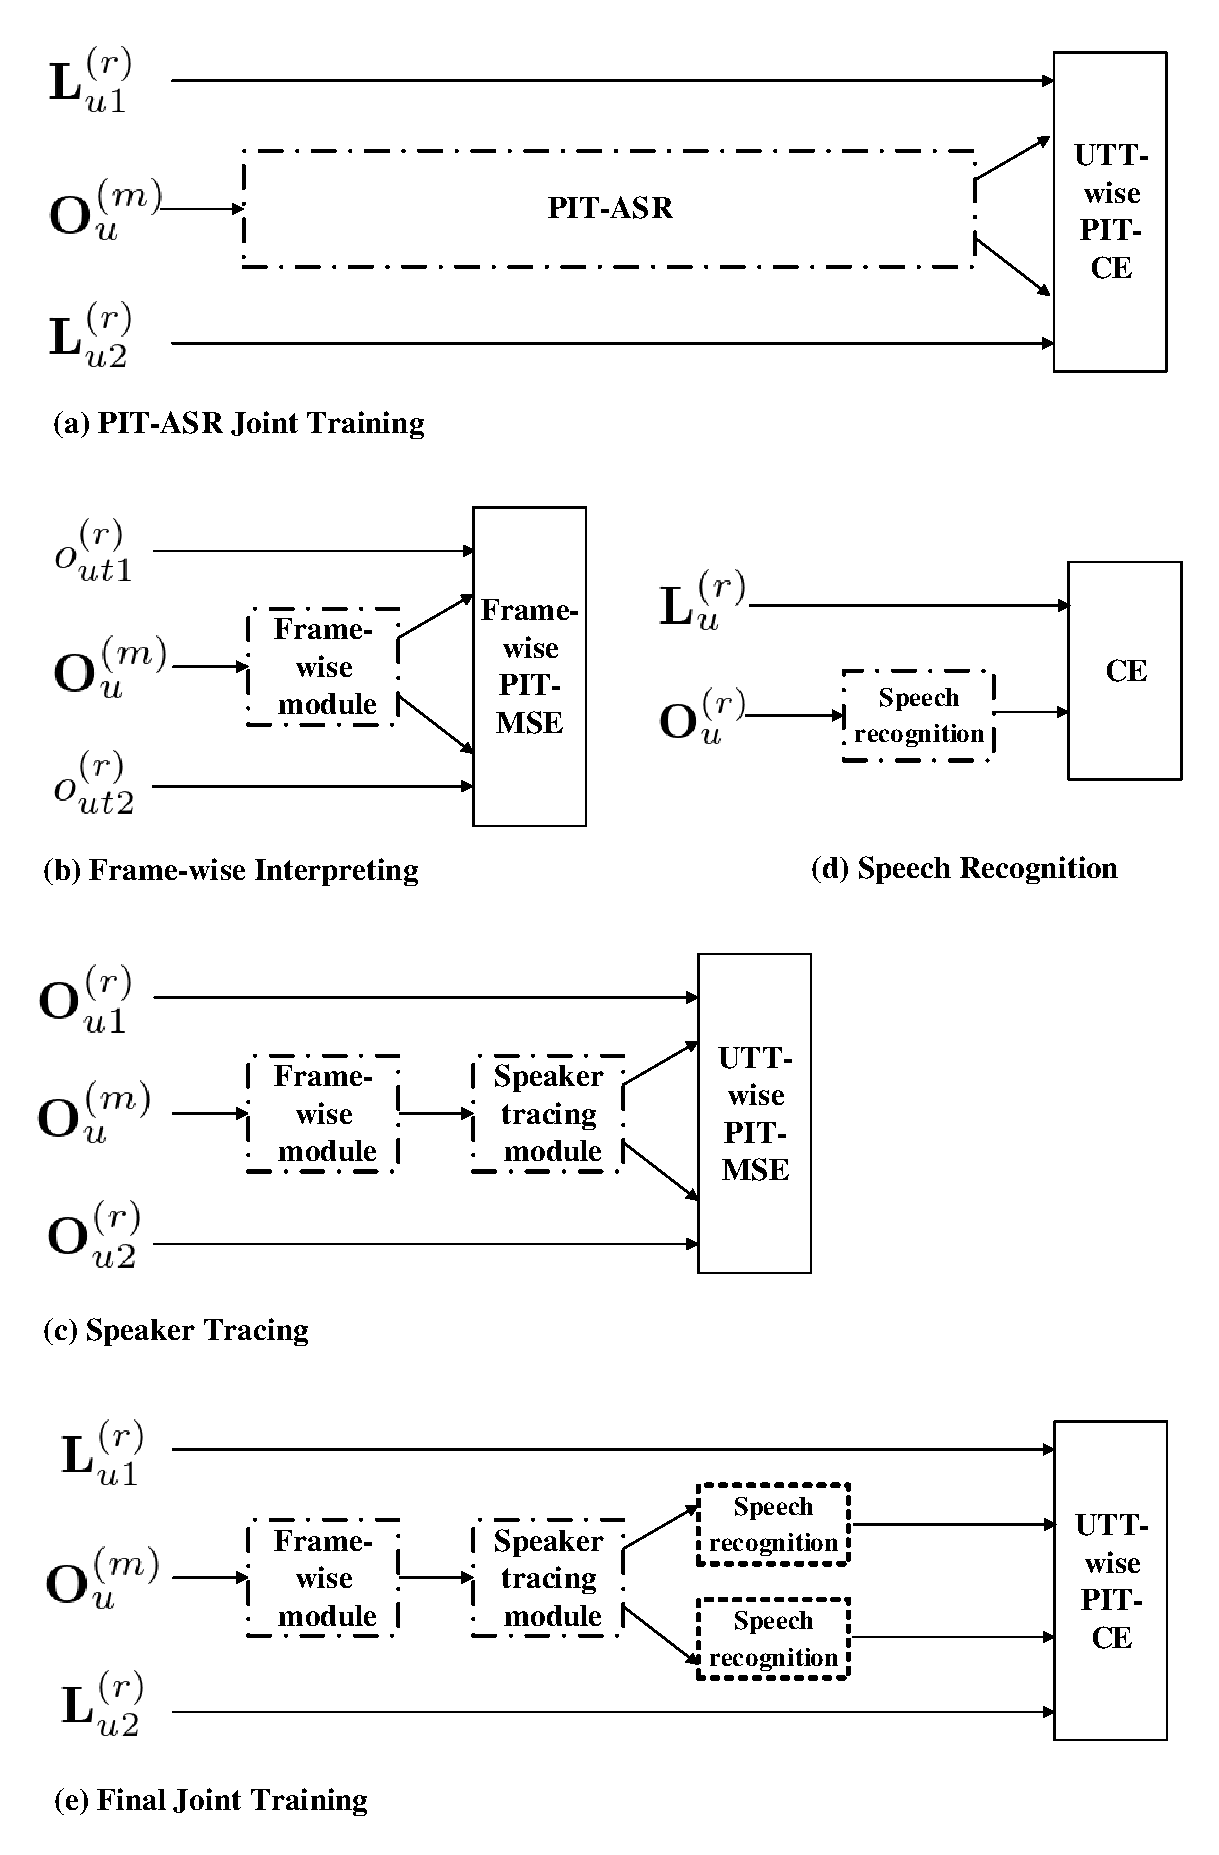
\includegraphics[width=0.7\linewidth]{figure/modules.pdf}
    \caption{\it PIT-ASR 联合训练与模块化初始化和逐步联合训练比较。 点划线框表示可以学习的模型参数。点线框表示可以学习的并且是共享模型参数。
    %The black blocks indicate the model parameters and the green blocks indicate the training criteria.
    }
    \label{fig:modules}
\end{figure*}

\subsection{基于迁移学习的排列不变性训练}
\label{chap:intro2-pit-ts}

迁移学习(教师-学生训练)被引入到这个问题中,以便使用平行干净语料来改善目标领域的混合语音识别系统。在这一框架中,学生是指该多说话人语音识别系统。它工作在目标领域,即混合语音信号的数据上,并尝试得到每个说话人相应的话语内容。这里教师模型输入源领域,即干净语音信号的,并尝试分别对每个说话人得到相应推理序列。


\begin{figure*}
  \centering
    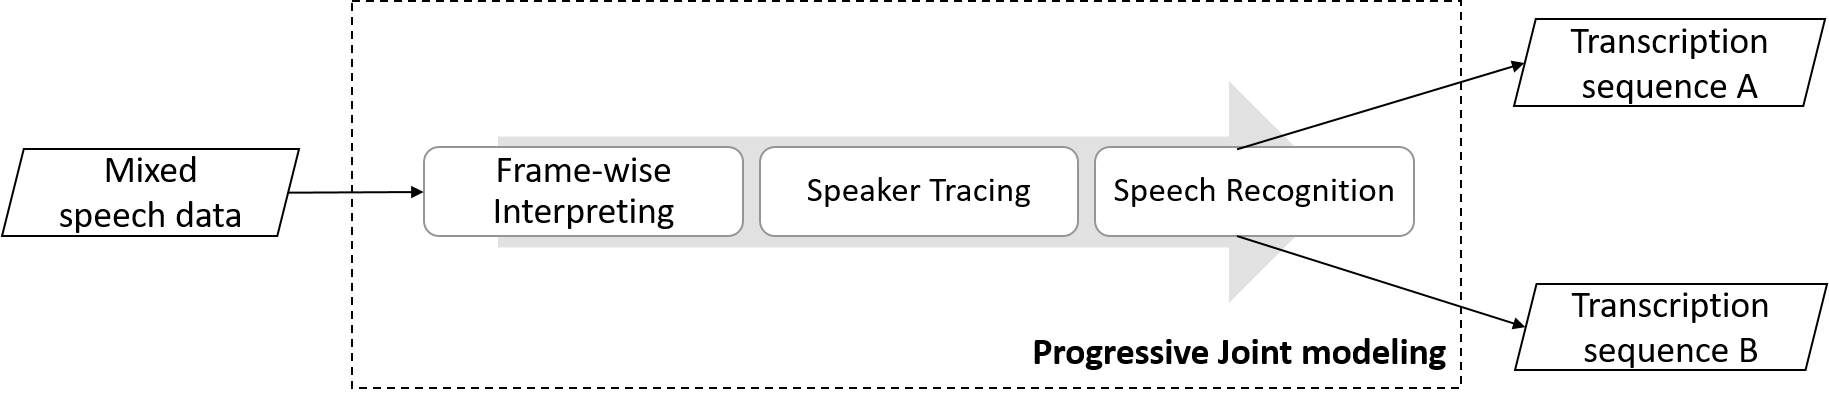
\includegraphics[width=0.8\linewidth]{figure/sys-framework.png}
    \caption{\it 模型系统训练框架。
    \cite{yu2017recognizing}中提出的结构由虚线框部分表示,其用于推理出每个说话人的语音信号的信息。该结构被模块化(三个实线框)并作逐一增量预训练。针对自身的迁移学习和多输出序列鉴别性训练在模块初始化后神经网络上进行。}
    \label{fig:sys-fr}
\end{figure*}


这一针对自身的迁移学习将最小化混合语音信号的模型和干净语音信号的模型输出分布之间的KL散度(KLD)。
这一KL散度被定义为句子层面干净语音信号的和混合语音信号的推理分布之间PIT准则,如下所示,
\begin{equation}
\label{equ:kld-opt}
\begin{split}
\mathcal{J}_{\text{KLD-PIT}}=\sum_u \min_{s'\in \mathbf{S}} \sum_t \frac{1}{N} \sum_{n\in[1,N]} \\
KLD(P({l}_{utn}^{(c)}|\mathbf{O}_{un}^{(r)}),P({l}_{utn}^{(s')}|\mathbf{O}_{u}^{(m)}))
\end{split}
\end{equation}
该式中,每个 $KLD(\cdot)$ 对的计算过程和经典领域自适应方式迁移学习公司相似。值得注意的一点是,当该方法被应用到如图~\ref{fig:joint-tr}所示的结构时,语音识别模块可以直接使用教师模型进行初始化。
% fixed [jasha] I think this sentence captures the meaning of the commented-out text below it.
% [t-zhehch] but we should define $P({l}_{utn}^{(s')}|\mathbf{O}_{u}^{(m)})$$ and $P({l}_{utn}^{(c)}|\mathbf{O}_{un}^{(r)})$
%Specifically, the clean speech model fine-tunes its parameters with other joint-trained modules in overlapped speech,  , to fit its own distribution in the simultaneous clean speech, i.e. clean speech model distribution .

图~\ref{fig:tr-curve}给出了多种训练方法在验证集上学习曲线比较。从图中可以看出,本章节所提出的方法具有更好初始点和最终的收敛点。这些都得益于本章节方法使得神经网络的学习任务更简单,最终收敛效果相应得到了提升。

\begin{figure}
  \centering
    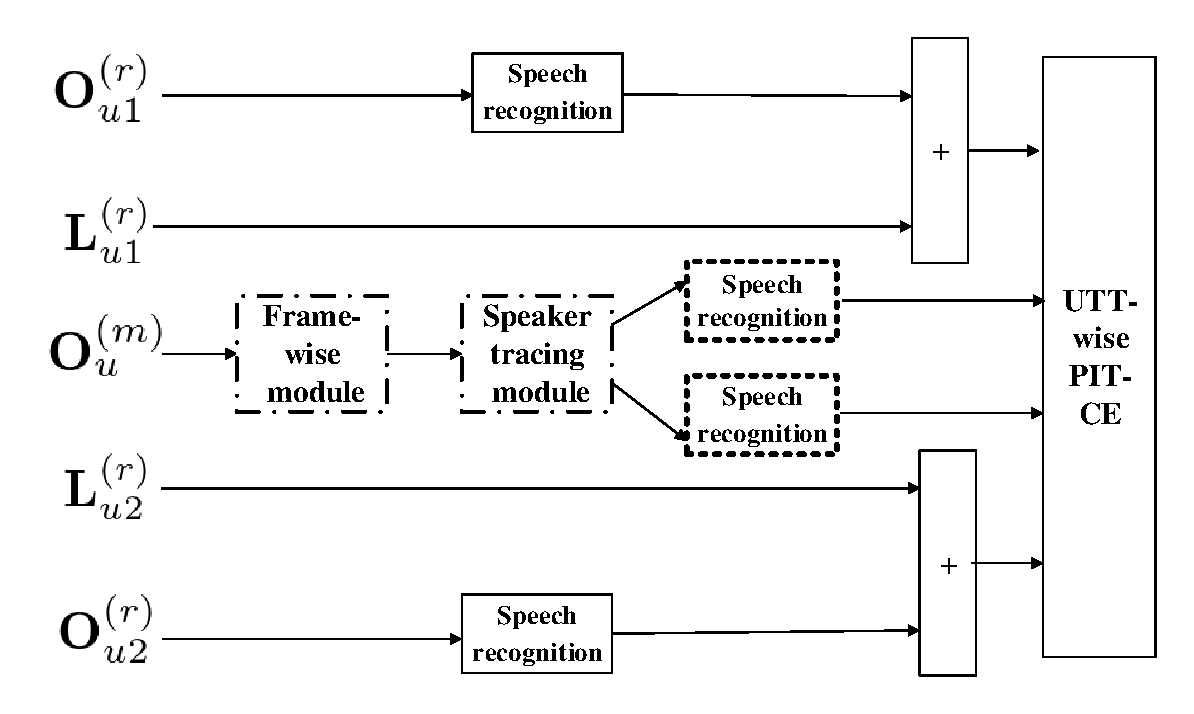
\includegraphics[width=\linewidth]{figure/joint-tr.pdf}
    \caption{\it 基于迁移学习逐步联合训练方法。点划线框表示可以学习的参数,点线框表示可以学习并且是共享模型参数。}
    \label{fig:joint-tr}
\end{figure}


\begin{figure}
{
  \centering
    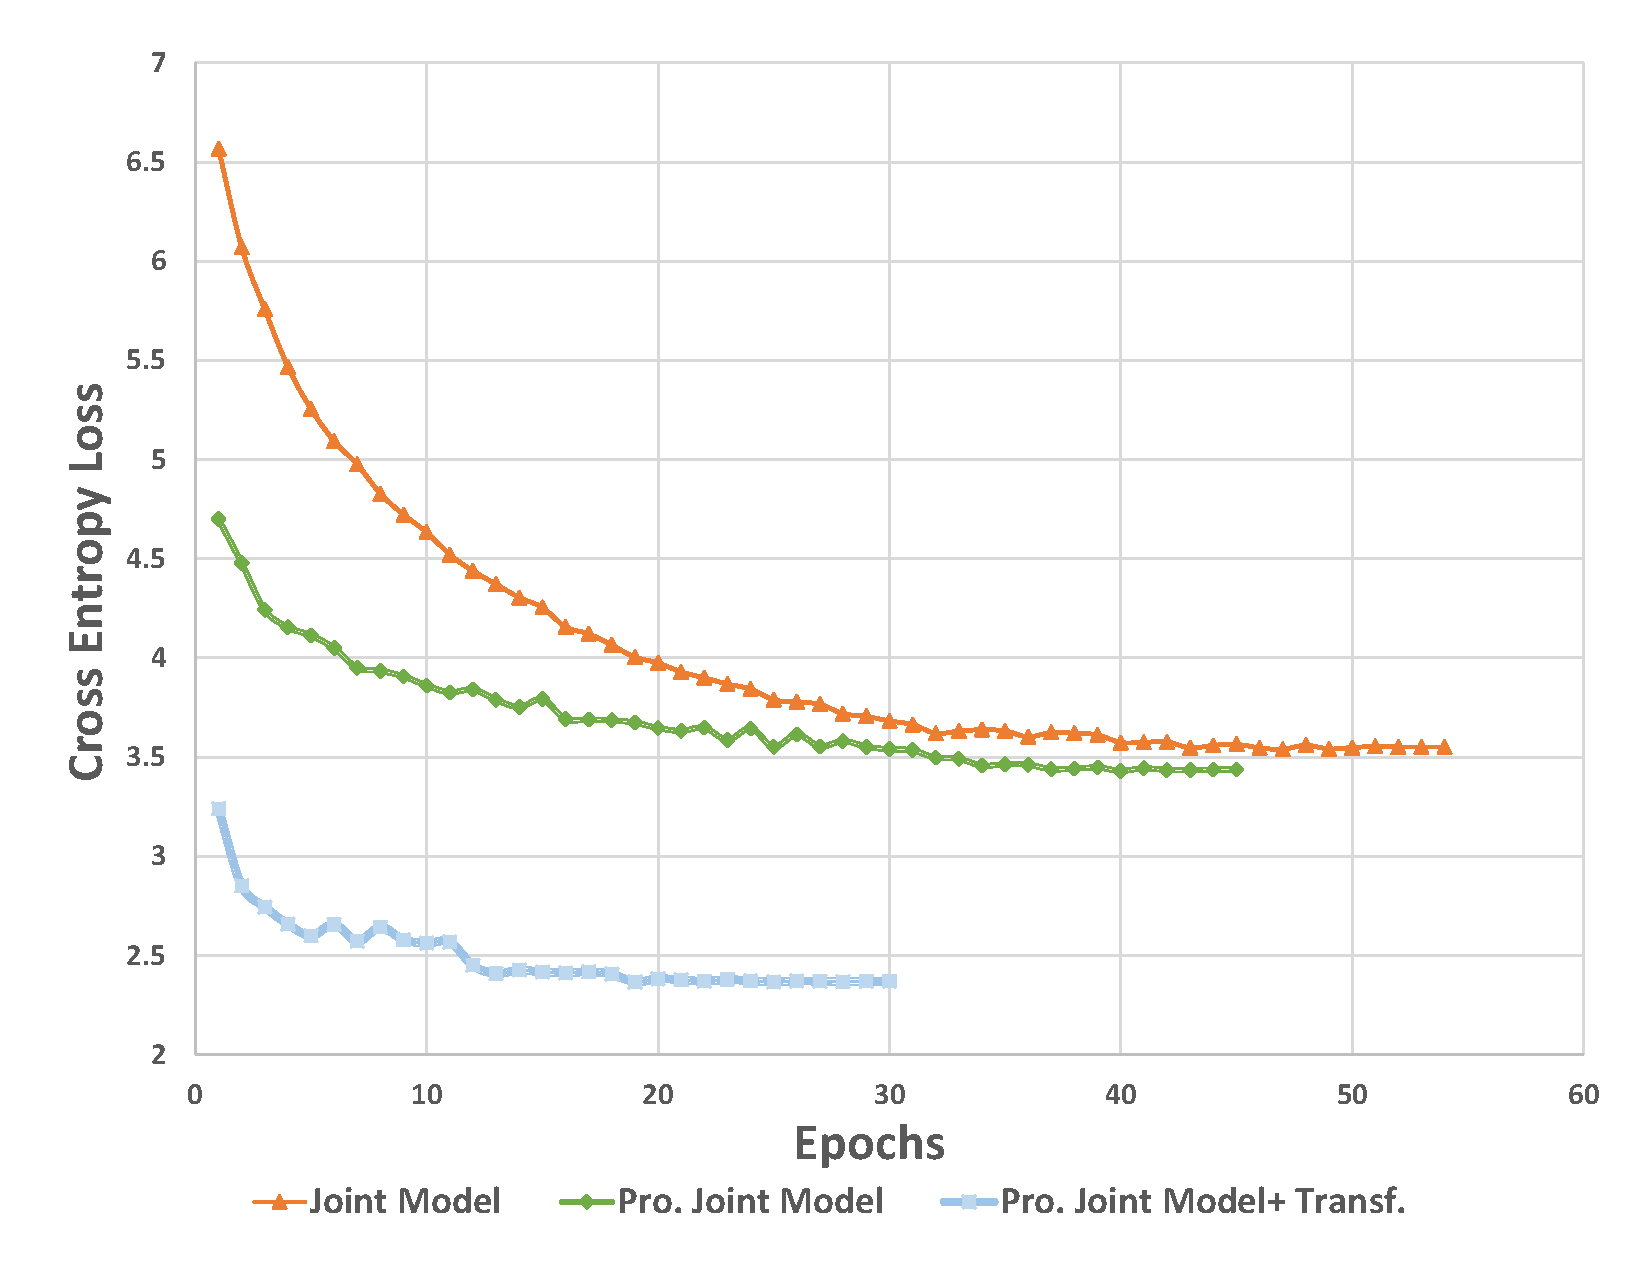
\includegraphics[width=\linewidth]{figure/tr-curve.pdf}
    }
    \caption{\it 原始联合训练和所提出的方法在验证集上学习曲线比较。在图中,联合训练,逐步联合训练,基于迁移学习逐步联合训练被分别表示为Joint Model,  Pro. Joint Model 和 Pro. Joint Model + Transf. 图中每个epoch包含24小时训练数据。 } 
    \label{fig:tr-curve}
\end{figure}

\subsection{基于序列鉴别性训练的排列不变性训练}
\label{chap:intro2-pit-dt}

本章节我们提出了一种传统鉴别性训练技术变种,它在进行鉴别性训练的同时,也抑制输出通道上说话人跟踪错误。

语音识别是一种序列分类和预测问题。因此在单输出语音识别中,序列级的准则将有助于改善系统性能。
而在鸡尾酒会问题中,对于单通道多说话人混叠语音识别系统,则又包含了说话人跟踪问题,也属于序列级问题。因此序列鉴别性准则将有助于这样序列分类问题。
在单输出语音识别中,我们使用如下公式对序列后验概率进行建模,

%ASR can be formulated as a {\em{maximum a posterior}} (MAP) decision process to integrate sequence level criteria to the training of the acoustic model. 
  
\begin{equation}
\label{equ:single-mbr}
\begin{split}
P(\mathbf{L}_u|\mathbf{O}_u)=\frac {p(\mathbf{O}_u|\mathbf{L}_u)P(\mathbf{L}_u)}{p(\mathbf{O}_u)}  
%y_{ut}(s^{(r)}_{ut})
\end{split}
\end{equation}
公式中$\mathbf{L}_u$ 是句子 $u$的词序列。 $P(\mathbf{L}_u)$ 是语言模型概率。
$p(\mathbf{O}_u|\mathbf{L}_u)$ 是相应声学模型概率。
 $p(\mathbf{O}_u)$ 是针对特征序列 $\mathbf{O}_u$观察概率进行建模的边缘概率,它等于所有可能的识别序列的概率求和。

通常来说,语言模型搜索空间是通过训练集语料来估计得到。之后在该搜索空间上将计算相应的序列准则。 
由于之前训练语料未出现词语交换问题,因此搜索空间也不包含这些建模。在这样搜索空间上训练将导致估计不准确,而最终的推测序列中将会增加较多词语交换错误。我们提出了一系列方法以解决该问题,这里想法是将词语交换错误添加到搜索空间中,由此减轻问题。
\begin{equation}
\label{equ:lf-dc-mmi}
\begin{split}
\mathcal{J}_{\tt{LF\text{-}DC\text{-}MMI}}
%=- \sum_{u} \log \frac {p(\mathbf{O}_u|\mathbf{S}_u)^{\kappa}P(\mathbf{L}_u)}{\sum_{\mathbf{L}} p(\mathbf{O}_u|\mathbf{S})^{\kappa}P(\mathbf{L})}  
=\sum_{u} \log  [ \frac {\sum_{\mathbf{L}_u} p(\mathbf{O}_u|\mathbf{L}_u)^{\kappa}P(\mathbf{L}_u)}{(\ \sum_{\mathbf{L}} p(\mathbf{O}_u|\mathbf{L})^{\kappa}P(\mathbf{L})\ )^{1-\lambda} } 
\cdot \\ 
\frac{1} {(\ {\sum_{\mathbf{L}_{\hat{u}}}} p(\mathbf{O}_u|{\mathbf{L}_{\hat{u}}})^{\kappa}P({\mathbf{L}_{\hat{u}}})\ )^\lambda}
 ]
\end{split}
\end{equation}
在公式~\ref{equ:lf-dc-mmi}中, 除当前优化的输出序列之外其他输出序列表示为 $\mathbf{L}_{\hat{u}}$。公式中添加了一项插值系数 $\lambda$。该部分额外式子最后被加入到分母优化当中。

% TODO
%\section{实验结果}
%\label{chap:intro2-exp}
%\subsection{端到端的大词汇连续语音识别}
%\label{chap:intro2-exp-e2e}
%\subsection{单通道多说话人鲁棒语音识别}
%\label{chap:intro2-exp-pit}
\section{本章小结}
\label{chap:intro2-sum}


在本章中,首先回顾了语音识别中最常用神经网络结构,主要包括深度神经网络、卷积神经网络、循环神经网络。接着探讨了神经网络的训练方法,包括训练准则、反向传播算法以及一些实际优化细节。随后回顾了深度神经网络-隐马尔可夫模型混合系统,这是目前语音识别领域最有效的将DNN与HMM结合的办法。
接着引出了目前研究的热点,即端到端语音识别系统。我们系统介绍了端到端建模各个变种,它们的特点及优势,为之后几章改进和推理框架研究进行了铺垫。最后我们介绍了基于深度序列模型的鲁棒语音识别及其在鸡尾酒会问题中几项研究。
